\chapter{从可见度到成像：角直径、多基线与 uv 覆盖}
\label{chap:e11}

\begin{chapteropening}
上一章我们把两台相距很远的望远镜连在一起，证明了它们记录的强度涨落是否同步，直接给出天体在某条基线上的平方可见度 \(|V(B)|^2\)——一个介于 0 和 1 之间的纯数字。可是天文学家要的从来不是一个数字，而是"这颗星有多大""它是圆的还是扁的""它是一颗星还是两颗贴在一起""表面有没有亮斑"，最终甚至是一张\emph{图}。本章要做的，就是把单条基线上那个孤零零的 \(|V|^2\) 一步步变成真正的科学产品：先算清楚"要测到这个数字，需要多亮的星、多大的镜子、多长的曝光"（信噪比）；再学会判断"这一夜的相关峰到底是真信号还是仪器捣鬼"（可行性与误差）；然后把两台望远镜扩成一个阵列，让地球自转帮我们在 Fourier 平面上画出一片二维覆盖（多基线与 uv 覆盖）；最后面对强度干涉与生俱来的软肋——相位丢了——看看闭合相位、相位恢复和物理先验怎样把图像重新拼回来。走完这一章，你会明白为什么一套 1960 年代被判"死刑"的老方法，会在今天的 Cherenkov 望远镜阵列上原地复活。
\end{chapteropening}

\section{要测到这个数字，得付出多少：强度干涉的信噪比}
\label{sec:e11-snr}

先把上一章的结论接住。对热光（thermal light，即普通恒星那种混沌光）而言，两台望远镜零延迟强度相关的超额，正比于该基线上的平方可见度；写成可以直接拟合观测数据的模型，就是第 \ref{chap:e10} 章得到的
\begin{equation}
  C_{12}(B)\equiv g_{12}^{(2)}(0)-1 = N_0\,f_1 f_2\,\big|V(B)\big|^2 ,
  \label{eq:e11-correlation-model}
\end{equation}
\begin{formulaexplain}
\(C_{12}\) 是基线 \(B\) 上测到的相关峰高度；\(N_0\) 是"零基线"仪器响应（源没被空间分辨时的聚束峰高）；\(f_1,f_2\) 是两台望远镜里目标光子占总计数的比例；\(|V|^2\) 是纯粹的天体结构项。仪器、背景、天体被干净地分成三段。
\end{formulaexplain}
这里 \(C_{12}\) 无量纲；\(N_0\) 也无量纲，量级在百万分之一（\(\sim10^{-6}\)）；\(f_1,f_2\) 是 0 到 1 之间的分数；\(|V(B)|^2\) 是我们真正想要的科学量。麻烦在于：这个信号\emph{实在太浅}。峰高只有 \(10^{-6}\) 到 \(10^{-3}\)，意味着我们要在一片几乎全是随机符合的背景上，去分辨百万分之一的一个隆起。能不能测到，取决于信噪比。

\paragraph{信噪比公式：逐个符号拆开}
\label{sec:e11-snr-formula}

Hanbury Brown 当年为 Narrabri 恒星强度干涉仪推导的双望远镜信噪比，今天仍是设计任何一次强度干涉观测的第一张算盘。它写成
\begin{equation}
  \left(\frac{S}{N}\right)_{\rm rms}
  = A\,\alpha\,n\,\big|\gamma_{12}\big|^2
  \left(\frac{\Delta f\,T}{2}\right)^{1/2}.
  \label{eq:e11-snr}
\end{equation}
\begin{formulaexplain}
\(A\) 是每台望远镜收集面积，\(\alpha\) 是探测效率，\(n\) 是光子谱流量，\(|\gamma_{12}|^2=|V|^2\) 是平方可见度，\(\Delta f\) 是电子带宽，\(T\) 是积分时间。信噪比\emph{线性}地跟着光子数走，却只按带宽和时间的\emph{平方根}长。
\end{formulaexplain}

这条式子每一个符号都值得单独交代，因为它们各自对应一个可以在设计观测时拧的"旋钮"：

\begin{itemize}
  \item \(A\)：每台望远镜的收集面积，单位 \({\rm cm^2}\)。这里为什么是 \(A\) 的\emph{一次}方，而不是 \(A^2\)？分子分母各走一步就清楚了：信号（那个符合计数超额）正比于两路总计数的乘积，也就是 \(\propto A_1 A_2\)；但噪声（散粒噪声底）也随两路的总计数一起涨，做除法时抵掉了一半的面积依赖，最后信噪比 \(\propto\sqrt{A_1 A_2}\)——两台等面积（\(A_1=A_2=A\)）时正好是一次 \(A\)，即两面积的\emph{几何平均}。换个等价说法：真正进入信噪比的物理量是每模式的占据数（简并度）\(\delta=A\,\alpha\,n\)，它本来就只带一次 \(A\)。抓住直觉即可：镜子越大，进来的目标光子越多，浅浅的相关峰就越站得住。
  \item \(\alpha\)：总光子探测效率，无量纲，是一串损失的乘积——镜面反射率 \(\times\) 滤光片透过率 \(\times\) 光电阴极量子效率 \(\times\) 读出/触发损失。典型现代蓝光系统 \(\alpha\sim0.2\)–\(0.3\)。
  \item \(n\)：目标在观测波段的\textbf{光子谱流量}（photon spectral flux），单位 \({\rm photons\,s^{-1}\,cm^{-2}\,Hz^{-1}}\)。它直接对应恒星的亮度——这是全式里唯一由"天上那颗星有多亮"决定、我们\emph{无法}用工程手段改变的量。
  \item \(|\gamma_{12}|^2=|V(B)|^2\)：这条基线上的平方可见度，无量纲，就是我们要测的科学量本身。注意信噪比正比于 \(|\gamma|^2\) 而非 \(|\gamma|\)：越靠近可见度零点、信号越弱的地方，越难测——这是强度干涉的宿命。
  \item \(\Delta f\)：电子相关带宽，单位 Hz，即相关器能分辨的最快时间结构 \(\sim1/\Delta f\)。注意它\emph{不是}光学滤光片带宽，而是探测器加电子学的响应带宽，现代系统在 \(10^8\)–\(10^9\,{\rm Hz}\)。
  \item \(T\)：积分时间，单位 s。
\end{itemize}

\paragraph{那个平方根是从哪儿来的}
\label{sec:e11-snr-sqrt}

式 \eqref{eq:e11-snr} 里最该讲清楚的，是括号里的 \((\Delta f\,T/2)^{1/2}\)——为什么信号明明是"测一个固定的相关峰高"，最后却冒出一个平方根？这不是魔法，而是第 \ref{chap:e03} 章那条"多次独立测量取平均，误差按 \(1/\sqrt{N}\) 缩小"的老结论在这里的直接兑现。我们把它一步步走出来。

\textbf{第一步：一次测量能独立采样多少次？}电子带宽 \(\Delta f\) 意味着相关器每隔约 \(1/\Delta f\) 的时间才能给出一个\emph{互相独立}的强度乘积样本（更快的结构它分辨不了，更慢的则被平滑掉）。于是在积分时间 \(T\) 里，独立样本的数目大约是
\[
  M \sim \Delta f\,T .
\]
取 \(\Delta f=1\,{\rm GHz}=10^9\,{\rm Hz}\)、\(T=5\,{\rm hr}=1.8\times10^4\,{\rm s}\)，就是 \(M\sim1.8\times10^{13}\) 次独立测量——一个天文数字。

\textbf{第二步：把 \(M\) 次独立测量平均起来。}每一次强度乘积的测量都被散粒噪声（shot noise）搞得上下乱跳，单次的信噪比极差。但它们彼此独立，于是按第 \ref{chap:e03} 章的中心极限结论，把 \(M\) 次取平均后，随机噪声的相对起伏缩小为原来的 \(1/\sqrt{M}\)。信号（那个真实的相关峰高）在平均中保持不变，噪声却被压低 \(\sqrt{M}\) 倍，所以
\[
  \frac{S}{N}\ \propto\ \sqrt{M}\ \sim\ \sqrt{\Delta f\,T}.
\]

\textbf{第三步：凑出前面的系数。}信号本身正比于\emph{被相关的目标光子率}，也就是 \(A\alpha n\)（面积 \(\times\) 效率 \(\times\) 谱流量）再乘上结构因子 \(|\gamma_{12}|^2\)；那个 \(1/\sqrt2\) 是热光两个偏振模式未被投影时的稀释因子（与上一章 \(N_0\sim1/(2\Delta\nu\Delta t)\) 里的同一个 \(1/2\) 同源）。把三步拼起来，就还原出式 \eqref{eq:e11-snr}。整个平方根的来历只有一句话：\emph{强度干涉靠的是在海量独立样本上做平均，而平均对随机噪声的压制，永远只有平方根那么快。}

\paragraph{两条必须记住的结论}
\label{sec:e11-snr-lessons}

式 \eqref{eq:e11-snr} 的结构里藏着两条会反复决定观测成败的经验：

\textbf{结论一：信噪比\emph{线性}地正比于光子谱流量、收集面积和效率。}三个因子 \(A\alpha n\) 都是一次方。这就是为什么强度干涉天生偏爱\emph{亮星}和\emph{大镜面}：星每暗一个星等，光子谱流量 \(n\) 就乘以 \(10^{-0.4}\simeq0.398\)，信噪比也直接打成四折；而把镜面口径从 \(6.5\,{\rm m}\)（Narrabri）换成 \(12\,{\rm m}\)（VERITAS），面积翻了 3.4 倍，信噪比同样翻 3.4 倍。天体的亮度我们改不了，但镜面和效率是工程能砸钱的地方——这正是"为什么要用大望远镜做强度干涉"的定量答案。

\textbf{结论二：信噪比只按 \((\Delta f\,T)^{1/2}\) 增长，慢得令人心痛。}平方根意味着\emph{曝光翻两番、信噪比才翻一番}：把观测从 5 小时加到 20 小时（\(\times4\)），信噪比只从比如 \(3\sigma\) 变成 \(6\sigma\)；把电子带宽从 \(250\,{\rm MHz}\) 提到 \(1\,{\rm GHz}\)（\(\times4\)），也只换来 2 倍。这解释了强度干涉长期的困境：想靠"多熬几夜"把暗星拉进探测范围，代价高得离谱；真正的突破口在结论一里那几个线性因子——更大的镜子、更高的效率、更亮的目标。

顺带说清一件常让初学者困惑的事：式 \eqref{eq:e11-snr} 里\emph{没有}光学滤光片带宽 \(\Delta\nu_{\rm opt}\)。这不是遗漏。关键是要记住 \(n\) 的定义（第 40 行那条）：它是\emph{每赫兹}的光子谱流量，量纲 \({\rm photons\,s^{-1}\,cm^{-2}\,Hz^{-1}}\)——它\emph{本身不随滤光片宽度变}。收窄滤光片，改变的是进来的\emph{总}光子数（\(\propto n\,\Delta\nu_{\rm opt}\)），而不是每赫兹的 \(n\)。那为什么总光子数少了、信噪比却不掉？因为在探测器远慢于光学相干时间的极限下（第 \ref{chap:e05} 章我们算过可见光 \(\tau_c<1\,{\rm ps}\)，而探测器响应在 ns 量级），收窄滤光片会同时按比例抬高相干时间 \(\tau_c\simeq1/\Delta\nu_{\rm opt}\) 与每模式的占据数（聚束峰 \(N_0\)）——总光子数下降与聚束峰上升在信噪比里恰好抵消。到头来，真正进入信噪比公式的只有\emph{与滤光片无关}的每赫兹谱流量 \(n\) 和电子带宽 \(\Delta f\)。所以窄带滤光片主要是用来\emph{压背景}的，不是用来提信号的——真实系统仍要把滤光片形状、背景和探测器响应老老实实塞进 \(N_0\) 或完整的似然函数里。

\begin{figure}[tbp]
\centering
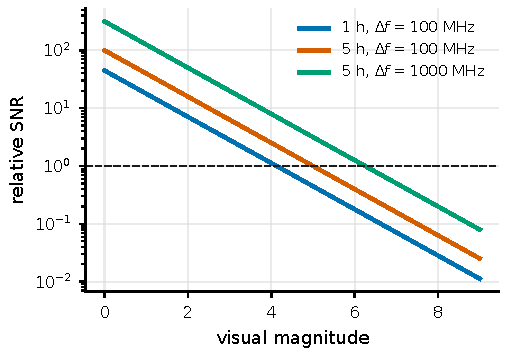
\includegraphics[width=0.86\linewidth]{figures/generated/chapter_05/ch05_snr_scaling.pdf}
\caption{强度干涉信噪比的相对标度。恒星每暗 1 等，光子谱流量约降为原来的 \(0.398\)，信噪比同比例线性下降；而积分时间和电子带宽只按平方根改善信噪比——曝光翻两番才换来信噪比翻一番。曲线未含收集面积、效率、背景稀释和 \(|V|^2\)，正是要凸显：亮星选择与高速电子学（线性因子）远比"多熬几夜"（平方根因子）划算。}
\label{fig:e11-snr-scaling}
\end{figure}

\paragraph{代入真实数字：Le Bohec--Holder 的数量级}
\label{sec:e11-snr-lebohec}

抽象公式要落地，就得代真实参数。Le~Bohec 和 Holder 在评估把 Cherenkov 阵列用于强度干涉的可行性时，做过一个经典估算 \citep{2006ApJ...649..399L}：取两台 \(A=100\,{\rm m^2}\) 的望远镜、探测效率 \(\alpha=0.3\)、电子带宽 \(\Delta f=1\,{\rm GHz}\)、积分时间 \(T=5\,{\rm hr}\)，在可见度平方 \(|\gamma_{12}|^2=0.5\) 的基线处，能以 \(5\sigma\) 显著性测到大约 \(V=6.7\) 等的恒星；对更亮的 \(V=5\) 等星，角直径精度可以做到几个百分点。对照上一节两条结论：这个 \(V=6.7\) 的极限灵敏度，几乎全由那几个线性因子（大面积、高效率、GHz 带宽）撑起来；想再往暗里推一等，靠的不是加时间（平方根，太贵），而是继续加面积和效率。

拿它和历史仪器对照，数量级立刻活了起来。Narrabri 用的是两台直径 \(6.5\,{\rm m}\) 的光收集器、\(443\,{\rm nm}\) 中心波长、\(10\,{\rm nm}\) 滤光片、光电阴极量子效率约 25\%、有效电子带宽仅约 \(60\,{\rm MHz}\) \citep{1967MNRAS.137..375H,1974MNRAS.167..121H,1974iiia.book.....H}。把这些数字代进式 \eqref{eq:e11-snr}，就明白为什么它的样本只能限于最亮的那批星（视星等大致 \(B<2.5\)）：面积比现代小、带宽小了一个多量级，几个线性和平方根因子叠加起来，把灵敏度死死钉在了亮星上。而 VERITAS 用四台 \(12\,{\rm m}\) 望远镜、250 MS/s 采样加离线相关，即使在接近满月、无法做伽马观测的"废时间"里，也能在几小时内测出恒星直径 \citep{2020NatAs...4.1164A}——这正是那几个线性因子（面积 \(\times3.4\)、效率提升）与更宽电子带宽联手的结果。

\section{怎样判断一次观测是真信号还是仪器捣鬼}
\label{sec:e11-feasibility}

信噪比公式告诉你"够不够亮、够不够久"，但它默认噪声是干净的白噪声。真实观测里最要命的敌人不是白噪声，而是两类会伪装成信号的东西：\emph{背景光}和\emph{系统相关}。因为真信号本身只有百万分之一到千分之一那么浅，任何一点没被识破的系统效应，都可能把角直径拟合带进沟里。

\paragraph{背景以两种方式同时伤人}
\label{sec:e11-background}

月光、夜天光（night-sky background）、被展宽的点扩散函数（PSF）里混进的相邻星光、探测器暗电流——这些非目标光子统称背景。它们伤害观测的方式\emph{有两条，而且同时起作用}：

\textbf{第一条，增加散粒噪声。}背景光子也要被探测、也要参与符合计数，它们贡献的散粒噪声直接抬高式 \eqref{eq:e11-snr} 分母里的噪声底，把信噪比往下拽。

\textbf{第二条，乘一个 \(f_1f_2\) 稀释因子。}回看式 \eqref{eq:e11-correlation-model}：相关峰被乘上了 \(f_1f_2\)，即两台望远镜里目标光子占总光子的比例之积。这一条更阴险，因为它是\emph{乘性}的。举个数字：若每台望远镜里目标光子只占 70\%（\(f_1=f_2=0.7\)），相关振幅就被压到
\[
  f_1 f_2 = 0.7\times0.7 = 0.49,
\]
只剩下不到一半。要把这半截信号找回同样的显著性，按信噪比的平方根标度，得把积分时间加到大约 4 倍——而积分越久，各种缓慢的系统漂移越容易冒头。Le~Bohec 和 Holder 早就指出，Cherenkov 望远镜那种 \(0.05^\circ\) 量级的宽光学 PSF 会让夜天光成为暗星灵敏度的边界；现代 VERITAS 的分析也必须专门修正夜天光背景和暗电流，否则角直径能被拉偏约 10\% 量级 \citep{2006ApJ...649..399L,2020NatAs...4.1164A,2025ApJ...995..191A}。这就是为什么窄带滤光片和小视场光阑在强度干涉里如此重要：它们不提信号，却是把 \(f_1,f_2\) 顶到接近 1 的关键。

\begin{figure}[tbp]
\centering
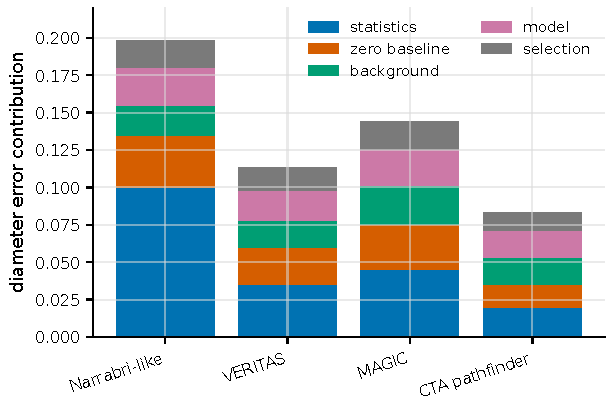
\includegraphics[width=0.82\linewidth]{figures/generated/chapter_05/ch05_error_budget.pdf}
\caption{强度干涉角直径误差预算的组成。统计误差（photon noise）会随光子数和积分时间按平方根下降，但零基线定标、背景稀释、恒星大气模型和天气/选择函数会共同筑起一道系统误差地板。现代阵列能不能出科学结果，取决于这些系统项能否和 photon noise 一起被诚实地写进似然函数——而不是被时间的平方根"熬"掉。}
\label{fig:e11-error-budget}
\end{figure}

\paragraph{系统相关比白噪声更危险}
\label{sec:e11-systematics}

白噪声至少是"公平"的：它随机，能靠平均压下去。真正让人夜不能寐的是\textbf{系统相关}（systematic correlation）——两路信号里某种\emph{非天体}的、却又同步的东西。地面反射、共用的时钟、电源纹波、温度联动、光纤串扰，都可能在两路电信号里注入一个假的相关峰。它之所以比白噪声危险，就因为真信号本来只有 \(10^{-6}\) 到 \(10^{-3}\)：白噪声再大，平均后也趋于零；而一个哪怕只有 \(10^{-5}\) 的系统相关，却不会被平均掉，它会稳稳地坐在那里，冒充成一个"可见度"。

对付它没有单一妙招，只有一整套交叉检验。下面这几条是强度干涉分析里的标准动作，值得当作检查清单背下来：

\begin{itemize}
  \item \textbf{远离零延迟处必须为零。}真正的热光聚束峰只出现在两路信号的\emph{时间对齐}处；把相对延迟拉到远离零的地方，相关应当归零。若那里还有残留，就是系统相关在作祟。
  \item \textbf{换通道或人为时移后峰应消失。}把两路信号互换、或故意插入一个不物理的时间偏移，真信号峰会随之移动或消失；如果峰纹丝不动，它就不是天上来的。
  \item \textbf{零基线响应 \(N_0\) 要处处一致。}用不同望远镜对、不同夜晚、不同月距、不同电子链路去测同一个"零基线"聚束高度，得到的 \(N_0\) 应当彼此吻合。\(N_0\) 一旦系统性偏移，式 \eqref{eq:e11-correlation-model} 里所有基线的 \(|V|^2\) 都会被整体拉伸，角直径、边缘昏暗、扁率全部跟着错。
  \item \textbf{\(|V|^2\) 应随\emph{基线}变，而不随电流变。}同一目标的可见度，只应当是投影基线 \(B\) 的函数；如果它反而跟着 PMT 阳极电流、环境温度或电子增益一起漂，那漂的就是仪器，不是恒星。
\end{itemize}

MAGIC 的强度干涉系统（MAGIC-SII）是把这套纪律工程化的好例子：它复用常规相机像素、加窄带滤光片、用 VCSEL 模拟光纤把信号传出、聚合电子带宽约 \(110\,{\rm MHz}\)、并用 GPU 实时无死时间（deadtime-free）相关器在线求相关，最终报告了 22 颗恒星的直径 \citep{2024MNRAS.529.4387A}。它把限制从"望远镜面积"推向了"工程稳定性与校准体系"——恰好印证：当信号浅到百万分之一，能不能压住系统相关，往往比镜子多大更决定成败。

\begin{figure}[tbp]
\centering
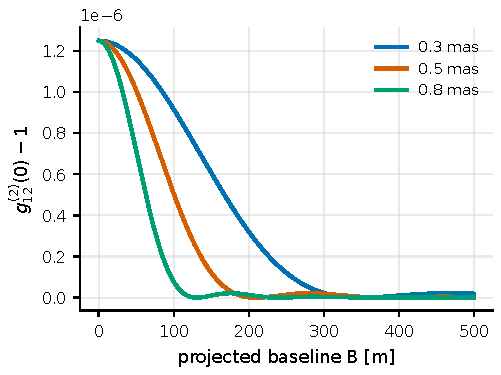
\includegraphics[width=0.86\linewidth]{figures/generated/chapter_05/ch05_sii_signal_vs_baseline.pdf}
\caption{用 \(C_{12}=N_0|V|^2\)（\(N_0\) 取 \(1.25\times10^{-6}\) 的现代蓝光系统量级）估算的强度干涉信号随基线的变化。角直径越大的星，\(|V|^2\) 越早随基线下降并出现零点；因此同一组基线对 0.8 mas 的星比对 0.3 mas 的星更敏感。观测设计的第一件事，就是照着目标的这条曲线，把基线摆在"下降区"——那里既有可观信号，又对角直径最敏感。}
\label{fig:e11-sii-signal}
\end{figure}

\section{从两台到一片：多基线与 uv 覆盖}
\label{sec:e11-uv}

两台望远镜，无论熬多久，也只能给你\emph{一条}投影基线上的一个 \(|V|^2\)。而上一章的 van~Cittert--Zernike 定理告诉我们，天体图像是它在整个 \((u,v)\) 平面上可见度的 Fourier 逆变换。所以要从"一个数字"走向"一张图"，唯一的出路是\emph{采到更多的空间频率}。这一节讲三件事怎样合力把采样从一个点铺成一整片。

\paragraph{望远镜数一多，基线数就爆炸}
\label{sec:e11-baseline-count}

第一件事最简单：多放望远镜。若阵列有 \(N\) 台望远镜，任取两台就构成一条基线，同时可形成的基线数是"从 \(N\) 里取 2"的组合数
\begin{equation}
  N_{\rm base}=\binom{N}{2}=\frac{N(N-1)}{2}.
  \label{eq:e11-baseline-number}
\end{equation}
\begin{formulaexplain}
\(N_{\rm base}\) 是可同时形成的望远镜对数（即基线数），\(N\) 是望远镜台数。每一对望远镜给一条独立基线，所以基线数随阵列规模近似按 \(N^2/2\) 爆炸式增长。
\end{formulaexplain}
组合数 \(\binom{N}{2}\) 的来历是标准计数：第一台有 \(N\) 种选法、第二台剩 \(N-1\) 种，但"甲乙"和"乙甲"是同一条基线要除以 2。代几个数就明白它多划算：\(N=2\) 只有 1 条基线；\(N=4\)（VERITAS）一下子有 6 条；\(N=17\) 有 136 条；而 CTAO 级别的几十到上百台望远镜，能同时给出上千条基线。基线数按 \(N^2\) 涨，是阵列望远镜相对双天线的根本优势。

这里要点出强度干涉一个\emph{独有}的甜头。振幅干涉（amplitude interferometry）要把同一束相干光在光学上分给多个合束器，每分一路就损失一份光子，路数一多信号就摊薄了。强度干涉不在光学上合束，它先把每台望远镜的光探测成\emph{电信号}，而电信号可以\textbf{无损地复制}到任意多个相关器里。于是一台望远镜的信号可以同时和其余每一台去求相关，把全部 \(N(N-1)/2\) 条基线一次拿下，完全不用在望远镜之间"分光"。对追求密集 \((u,v)\) 覆盖的成像来说，这是强度干涉方案天然的便宜。

\paragraph{让地球替你转：一条基线扫出一段轨迹}
\label{sec:e11-earth-rotation}

第二件事不花一分钱：等地球自转。一对望远镜在地面上的间隔矢量是固定的，但它\emph{投影到垂直视线的天空平面}上的分量，会随目标在天上升落而不断改变。回忆上一章的定义，空间频率就是投影基线除以波长，\(u=B_x/\lambda,\ v=B_y/\lambda\)。随着地球把目标从东边转到西边，投影基线 \((B_x,B_y)\) 连续变化，于是同一对固定的望远镜，会在一夜之内让它的采样点\emph{沿着 \((u,v)\) 平面画出一段弧线}。这套"地球自转合成孔径"（Earth-rotation synthesis）是射电干涉几十年的看家本领，在强度干涉里同样适用：只要每隔几分钟就把相关结果存一次，一个采样点就被拉成了一条轨迹。

\paragraph{多夜、多时角、多望远镜对：拼出二维覆盖}
\label{sec:e11-2d-coverage}

第三件事是把前两件反复叠加。一夜之内地球只能转过一段时角（hour angle），画出的弧线有限；但换一夜、换一个季节、把目标在不同时角下都观测一遍，弧线就一段段接上。再把阵列里\emph{每一对}望远镜的轨迹全叠在同一张 \((u,v)\) 图上——每对望远镜画一条、加上它关于原点对称的共轭点（因为真实亮度分布保证 \(V(-u,-v)=V^*(u,v)\)，负频率点同样是约束）——最终就从零零星星几个点，拼出一片二维的 \((u,v)\) 覆盖。覆盖越稠密，能区分的天体结构就越精细：稀疏采样只够拟合一个直径，稠密采样才能分辨圆盘、椭圆、双星，乃至表面亮斑 \citep{2008AIPC..984..205L,2012MNRAS.419..172N,2013APh....43..331D}。

\begin{figure}[tbp]
\centering
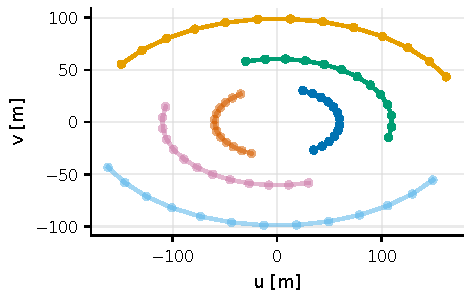
\includegraphics[width=0.82\linewidth]{figures/generated/chapter_05/ch05_uv_coverage.pdf}
\caption{固定的望远镜基线在地球自转中被投影到不同的 \((u,v)\) 位置。每条彩色轨迹代表一对望远镜在一夜时角变化中扫过的空间频率，原点对称的共轭点（虚线一侧）也是对实亮度分布的有效 Fourier 约束。多对望远镜、多夜、多时角叠加起来，采样就从孤立几点长成二维覆盖——覆盖越密，越能把圆盘、椭圆、双星和表面斑点区分开。}
\label{fig:e11-uv-coverage}
\end{figure}

\section{相位丢了怎么办：闭合相位、相位恢复与低维模型}
\label{sec:e11-phase}

到这里必须直面强度干涉与生俱来的软肋。振幅干涉直接测复可见度 \(V=|V|e^{i\phi}\)，模和相位一起拿到；而强度干涉只测\emph{强度涨落的同步程度}，得到的是 \(|V|^2\)——\textbf{相位 \(\phi\) 丢了}。这不是小事：Fourier 相位恰恰编码着"亮度往哪边偏"的信息。丢了相位最直接的后果是一种镜像退化——一个亮度分布 \(I(l,m)\) 和它的中心反演镜像 \(I(-l,-m)\)，拥有\emph{完全相同}的 \(|V|^2\)，光凭平方可见度永远分不开这两者。只测模平方，等于只知道每个空间频率上"有多少起伏"，却不知道"起伏的相位对齐在哪"。要重建真正的图像，就得设法把相位信息补回来。有三条路。

\paragraph{出路一：三阶闭合相位}
\label{sec:e11-closure}

第一条路承接第 \ref{chap:e08} 章的三阶相干函数 \(g^{(3)}\)。当年那条三阶公式落到三台望远镜 \(1,2,3\) 上时，会冒出一项
\begin{equation}
  2\,{\rm Re}\big(\gamma_{12}\,\gamma_{23}\,\gamma_{31}\big),
  \label{eq:e11-triple}
\end{equation}
\begin{formulaexplain}
\(\gamma_{12},\gamma_{23},\gamma_{31}\) 是三条边上的复相干度。它们的乘积把三条边的相位加在一起：\(\phi_{12}+\phi_{23}+\phi_{31}\)。这个"绕三角形一圈"的相位和，就是闭合相位。
\end{formulaexplain}
关键在于这个三元乘积的相位。设每台望远镜因大气或仪器引入一个未知的"活塞"相位（piston）\(\psi_i\)，它会给每条边的相位加上 \(\psi_j-\psi_i\)。把三条边绕三角形转一圈相加：
\[
  (\psi_2-\psi_1)+(\psi_3-\psi_2)+(\psi_1-\psi_3)=0.
\]
每台望远镜那个讨厌的未知相位\emph{精确抵消}了！剩下的相位和 \(\phi_{12}+\phi_{23}+\phi_{31}\) 只属于天体本身，这个量叫\textbf{闭合相位}（closure phase）。它在概念上正是振幅干涉里对付大气抖动的老武器，如今在强度干涉里以三阶相关的面貌重现，且天然免疫单台望远镜的相位漂移。

天下没有免费的午餐：三阶信号比二阶弱得多。二阶靠的是光子\emph{成对}到达的关联，三阶要求光子\emph{三个一组}同时到达，而三元组比二元组稀罕太多，误差传播也更苛刻。所以闭合相位更适合超大阵列和极亮目标，而不是每次观测的默认产品。

\paragraph{出路二：二维覆盖 + 相位恢复算法 + 物理先验}
\label{sec:e11-phase-retrieval}

第二条路绕开相位测量，直接从一片稠密的二维 \(|V|\) 分布里\emph{反解}出相位。这听起来像无中生有，但数学上并非全无希望：对一个紧支撑（compact support）的实亮度分布，其 Fourier 模与相位并非完全独立，模的解析结构（经由 Cauchy--Riemann 关系）对相位施加了约束。Gerchberg--Saxton 迭代 \citep{1966JOSA...56..441G}、MIRA 之类的正则化重建算法，就是在"符合测到的 \(|V|\)"和"满足物理先验"两个约束之间来回投影，逼出一个自洽的相位。这里的\textbf{物理先验}是命门：亮度非负、源有有限大小、亮度分布光滑、必要时套一个恒星大气模板——正是这些先验把镜像退化和无穷多的伪解筛掉。Nuñez 等人的模拟表明，在 CTA 级别的 \((u,v)\) 覆盖下，明亮热星、快速自转星、双星、带表面斑点的恒星都能被恢复到有物理意义的形状参数，但成败取决于信噪比、短基线覆盖是否足够、先验掩膜和图像正则化怎么设 \citep{2012MNRAS.419..172N,2012MNRAS.424.1006N,2014SPIE.9146E..0ZD}。

\paragraph{出路三：干脆不重建图像，用低维模型}
\label{sec:e11-low-dim}

第三条路最务实，也常常最有力：\emph{根本不做无模型的图像重建}，而是拿一个只有几个参数的物理模型去拟合 \(|V|^2\)。别忘了，只测 \(|V|^2\) 绝不等于只能测直径。对一大类低维模型——均匀圆盘（uniform disk）、椭圆圆盘、双星、边缘昏暗（limb darkening）——平方可见度已经能给出\emph{很强}的约束。均匀圆盘的可见度是 \(V(B)=2J_1(x)/x\)（\(x=\pi\theta B/\lambda\)，第 \ref{chap:e10} 章由 Bessel 函数第一零点 \(x=3.8317\) 定出角直径），扁椭圆会让零点基线随方位角变化，双星会在 \(|V|^2\) 上叠一层余弦振荡，边缘昏暗会把第一 lobe 的形状微微改样。这些差异都\emph{不需要相位}就能从 \(|V|^2\) 曲线里读出来。当科学目标是"这颗星多大、多扁、是不是双星"，而不是"给我一张模型无关的照片"时，几个参数的模型往往比费劲的相位恢复更稳、更可信。

\section{一套老方法为什么会复活：从 Narrabri 到 CTAO}
\label{sec:e11-history}

把前面所有工具串起来，就能看懂强度干涉这条曲折的技术史——它曾被判死刑，又在半个世纪后原地复活。

\textbf{Narrabri（1960s--1970s）：证明这条路走得通。}澳大利亚 Narrabri 的恒星强度干涉仪（Stellar Intensity Interferometer）是第一台完整展示这套方法科学能力的仪器。两台直径 \(6.5\,{\rm m}\) 的光收集器在 10--188 m 的可变轨道基线上工作，滤光片中心约 \(443\,{\rm nm}\)、带宽 \(10\,{\rm nm}\)，光电阴极量子效率约 25\%，有效电子带宽约 \(60\,{\rm MHz}\)。它测出了 32 颗恒星的角直径和若干双星，最小直径约 \(0.4\,{\rm mas}\) \citep{1967MNRAS.137..375H,1967MNRAS.137..393H,1974MNRAS.167..121H,1974iiia.book.....H}。但它随后停用，原因恰好是式 \eqref{eq:e11-snr} 里那几个线性因子当年都上不去：可移动的大面积光收集器造价高、低噪声高速电子学不成熟、又缺乏多基线成像能力。老方法不是错了，是当时的硬件配不上它。

\textbf{VERITAS（2019--）：老思想撞上现成的大镜子。}转机来自大气 Cherenkov 望远镜阵列。它们本是为捕捉伽马射线引发的纳秒级 Cherenkov 闪光而造，天然就有 10~m 级口径、大面积镜面、快速 PMT、长基线和可接受的光学像质——恰好是强度干涉当年求之不得的一切。VERITAS 用四台 \(12\,{\rm m}\) 望远镜同时形成 6 条基线，对 \(\beta\)~CMa 和 \(\epsilon\)~Ori 测得均匀圆盘直径 \(\theta_{\rm UD}=0.523\pm0.017\,{\rm mas}\) 和 \(0.631\pm0.017\,{\rm mas}\)，精度优于 5\%，只用了几小时，而且是在接近满月、无法做伽马观测的时段里"顺手"完成的 \citep{2020NatAs...4.1164A}。随着 \((u,v)\) 覆盖改善，它对 \(\beta\)~UMa 和快速自转星 \(\gamma\)~Cas 的后续观测，已经从"测一个半径"进到"测方向依赖的形状"：\(\gamma\)~Cas 用 6 条基线、超过 160 pair-hours 的数据测出可见光球的扁率，小轴直径约 \(0.43\,{\rm mas}\)、长短轴比约 1.28、自转轴位置角约 \(116^\circ\) \citep{2024ApJ...966...28A,2025ApJ...995..191A}。

\textbf{MAGIC-SII（2024）：把它变成一个可切换的标准模式。}MAGIC 用两台 \(17\,{\rm m}\) 抛物面望远镜、复用原有相机像素，配上 VCSEL 模拟光纤传输和 GPU 实时无死时间相关器（聚合带宽约 \(110\,{\rm MHz}\)），实现了在常规伽马观测与强度干涉模式之间快速切换，并报告了 22 颗恒星的直径 \citep{2024MNRAS.529.4387A}。它示范的不只是"能测"，而是"能作为一台成熟设备的常规副业稳定运行"。

\textbf{CTAO（在建）：走向公里基线与上千条基线。}下一代的 CTAO 把强度干涉的两大杠杆同时拉满。公里级基线在 350--450 nm 对应\emph{几十微角秒}的分辨率——比 Narrabri 精细一两个量级；而几十到上百台望远镜按式 \eqref{eq:e11-baseline-number} 能给出\emph{上千条}基线和极密的 \((u,v)\) 覆盖，这正是第 \ref{sec:e11-phase} 节里相位恢复和图像重建赖以成功的前提。它不会取代 CHARA、VLTI 那样的振幅干涉仪——灵敏度、相位能力和红外波段各有专长——而是成为一件互补的利器：专攻蓝光、超长基线、亮热星与快速变化天体 \citep{2013APh....43..331D,2014SPIE.9146E..0ZD}。

一句话收束这段历史：老方法之所以复活，不是因为思想变了，而是因为式 \eqref{eq:e11-snr} 里那几个线性因子（面积、效率、带宽、基线数）终于被 Cherenkov 阵列一次性喂饱了。物理一直在那里等着，是硬件姗姗来迟。

\section{本章要点}
\label{sec:e11-summary}

\begin{itemize}
  \item \textbf{信噪比公式是第一张算盘。}\((S/N)_{\rm rms}=A\,\alpha\,n\,|\gamma_{12}|^2(\Delta f\,T/2)^{1/2}\)：那个平方根来自"在 \(M\sim\Delta f\,T\) 个独立样本上取平均、噪声按 \(1/\sqrt{M}\) 缩小"（第 \ref{chap:e03} 章）。
  \item \textbf{两条结论要背下来。}信噪比\emph{线性}正比于光子谱流量、面积、效率（亮星、大镜面是关键）；却只按 \((\Delta f\,T)^{1/2}\) 增长（曝光翻两番才换信噪比翻一番）。改进要靠线性因子，不要指望多熬几夜。
  \item \textbf{背景两路伤人。}既增加散粒噪声，又把相关振幅乘上 \(f_1f_2\)（目标占比 70\% 就只剩 0.49）。窄带滤光片和小视场光阑是把 \(f_1,f_2\) 顶到接近 1 的关键。
  \item \textbf{系统相关比白噪声更危险，}因为真信号本就只有 \(10^{-6}\)–\(10^{-3}\)。标准检验：远离零延迟处相关应为零；换通道/人为时移后峰应消失；\(N_0\) 要处处一致；\(|V|^2\) 应随基线而非随电流变化。
  \item \textbf{多基线走向成像。}\(N\) 台望远镜给 \(N(N-1)/2\) 条基线；地球自转让每对基线扫过一段 \((u,v)\) 轨迹；多夜、多时角叠加拼出二维覆盖。强度干涉的独门便宜：电信号可无损复制到许多相关器，不必在望远镜间分光。
  \item \textbf{相位问题有三条出路。}三阶闭合相位（承接第 \ref{chap:e08} 章 \(g^{(3)}\)，piston 自动抵消，但信号弱）；二维覆盖 + 相位恢复算法 + 物理先验；以及最务实的——用均匀盘/椭圆盘/双星/边缘昏暗等低维模型，\(|V|^2\) 已能强约束形状。
  \item \textbf{老方法复活的定量原因：}Narrabri（\(6.5\,{\rm m}\)、443~nm、\(\sim60\,{\rm MHz}\)、测 32 星、最小 \(\sim0.4\,{\rm mas}\)）\(\to\) VERITAS（\(4\times12\,{\rm m}\)、\(\beta\)~CMa/\(\epsilon\)~Ori 精度 <5\%）\(\to\) MAGIC-SII（\(2\times17\,{\rm m}\)、GPU 相关器、22 星）\(\to\) CTAO（公里基线、几十微角秒、上千基线）。物理没变，是硬件把式 \eqref{eq:e11-snr} 的线性因子喂饱了。
\end{itemize}

\medskip
\noindent\textbf{想一想。}
\begin{enumerate}
  \item 一颗星比另一颗暗 2.5 个星等，其他条件相同，要测到同样的信噪比，积分时间大约要长多少倍？（提示：先用线性因子算信噪比降了几倍，再用平方根标度换算时间。）
  \item 一个 6 台望远镜的阵列能同时形成多少条基线？若再添 4 台凑成 10 台，基线数是原来的几倍？这对 \((u,v)\) 覆盖意味着什么？
  \item 为什么强度干涉能容忍很差的光学像质，却对电子学的时间对齐极其敏感？把它和"振幅干涉要求光程稳定到一小部分波长"对照，说说两者各自的"精度预算"花在了哪里。
\end{enumerate}
